\documentclass[tikz]{standalone}

\begin{document}
\begin{tikzpicture}[scale=1, node distance=10cm]

    \node[] (A) {
        \begin{tikzpicture}[y={(0.02cm,0.6cm)},x={(0.5cm,0cm)}, z={(-1cm, 0.5cm)}, scale=1]
            \draw[fill=gray!5]  (0, 0, -3) -- (8.5, 0, -3) -- (8.5, 11, -3) -- (0, 11, -3) -- cycle;
            \draw[fill=gray!15] (0, 0, -2) -- (8.5, 0, -2) -- (8.5, 11, -2) -- (0, 11, -2) -- cycle;
            \draw[fill=gray!25] (0, 0, -1) -- (8.5, 0, -1) -- (8.5, 11, -1) -- (0, 11, -1) -- cycle;
            \draw[fill=gray!35] (0, 0,  0) -- (8.5, 0,  0) -- (8.5, 11,  0) -- (0, 11,  0) -- cycle;
        \end{tikzpicture}
    };

    \node[below of=A] (B) {
        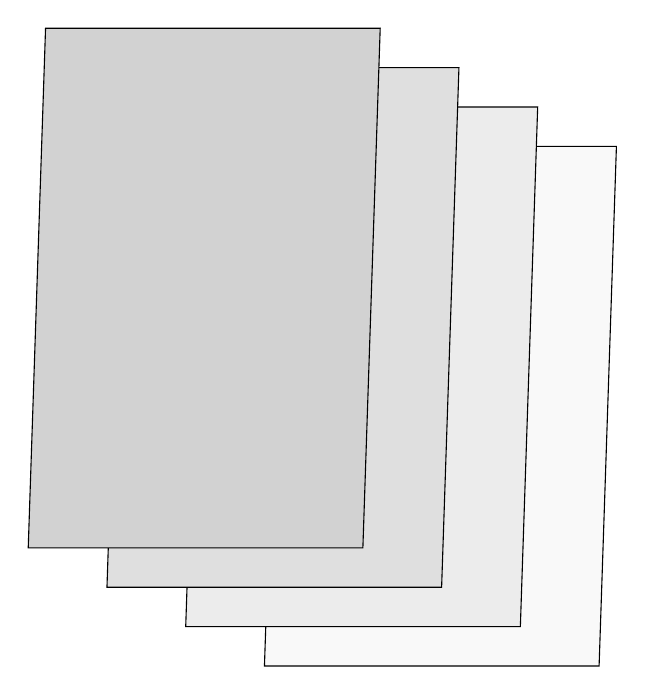
\begin{tikzpicture}[y={(0.02cm,0.6cm)},x={(0.5cm,0cm)}, z={(-1cm, 0.5cm)}, scale=1]
            \draw[fill=gray!5]  (0, 0, -3) -- (8.5, 0, -3) -- (8.5, 11, -3) -- (0, 11, -3) -- cycle;
            \draw[fill=gray!15] (0, 0, -2) -- (8.5, 0, -2) -- (8.5, 11, -2) -- (0, 11, -2) -- cycle;
            \draw[fill=gray!25] (0, 0, -1) -- (8.5, 0, -1) -- (8.5, 11, -1) -- (0, 11, -1) -- cycle;
            \draw[fill=gray!35] (0, 0,  0) -- (8.5, 0,  0) -- (8.5, 11,  0) -- (0, 11,  0) -- cycle;
        \end{tikzpicture}
    };

    \node[right of=B] (C) {
        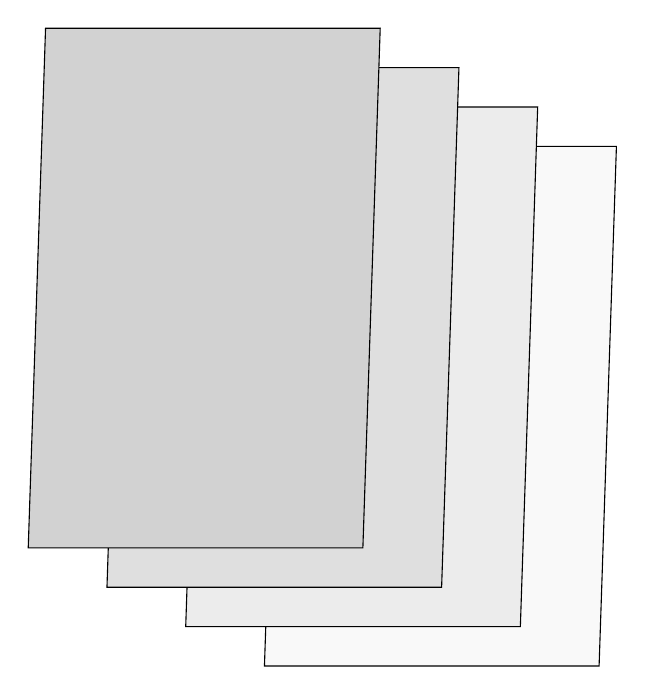
\begin{tikzpicture}[y={(0.02cm,0.6cm)},x={(0.5cm,0cm)}, z={(-1cm, 0.5cm)}, scale=1]
            \draw[fill=gray!5]  (0, 0, -3) -- (8.5, 0, -3) -- (8.5, 11, -3) -- (0, 11, -3) -- cycle;
            \draw[fill=gray!15] (0, 0, -2) -- (8.5, 0, -2) -- (8.5, 11, -2) -- (0, 11, -2) -- cycle;
            \draw[fill=gray!25] (0, 0, -1) -- (8.5, 0, -1) -- (8.5, 11, -1) -- (0, 11, -1) -- cycle;
            \draw[fill=gray!35] (0, 0,  0) -- (8.5, 0,  0) -- (8.5, 11,  0) -- (0, 11,  0) -- cycle;
        \end{tikzpicture}
    };

    \node[above of=C] (D) {
        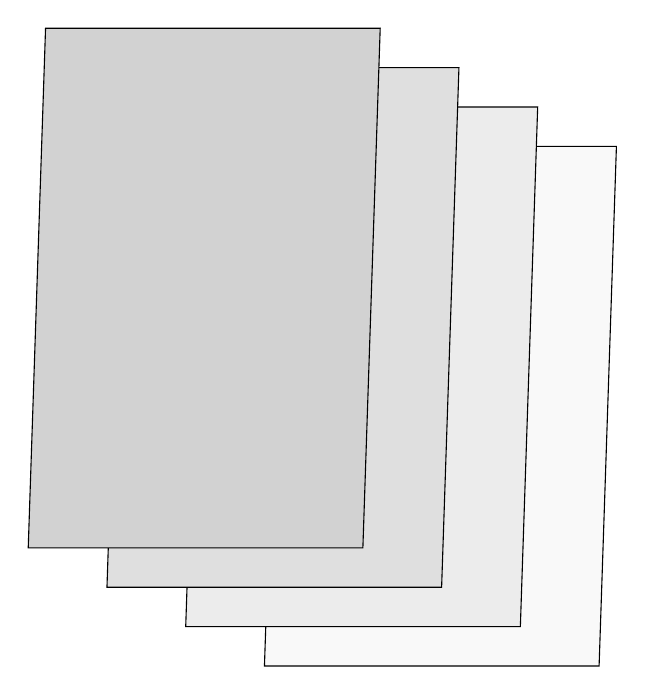
\begin{tikzpicture}[y={(0.02cm,0.6cm)},x={(0.5cm,0cm)}, z={(-1cm, 0.5cm)}, scale=1]
            \draw[fill=gray!5]  (0, 0, -3) -- (8.5, 0, -3) -- (8.5, 11, -3) -- (0, 11, -3) -- cycle;
            \draw[fill=gray!15] (0, 0, -2) -- (8.5, 0, -2) -- (8.5, 11, -2) -- (0, 11, -2) -- cycle;
            \draw[fill=gray!25] (0, 0, -1) -- (8.5, 0, -1) -- (8.5, 11, -1) -- (0, 11, -1) -- cycle;
            \draw[fill=gray!35] (0, 0,  0) -- (8.5, 0,  0) -- (8.5, 11,  0) -- (0, 11,  0) -- cycle;
        \end{tikzpicture}
    };

\end{tikzpicture}
\end{document}
